\chapter{O-C Diagrams and Simulations}
\label{ch:oc_sim}

In this chapter we briefly describe O-C diagrams as a method that we use for 
detection of $3^{rd}$ bodies (circumbinary planets or brawn dwarfs in our case) in eclipsing binary systems.
Also we present our simulation of $3^{rd}$ bodies in eclipsing binary systems.

\section{O-C diagrams}
Observed minus Calculated diagrams is a diagnostic tool and interpretation 
of the disagreement between the measure of an observable event and its predicted value \citep{Sterken2005basic}.
In astronomy, O-C diagram usually is used when discussing cyclic phenomena where the times of occurrence of a given event is irregular. 
The O-C diagram is then constructed by plotting the quantity O-C as a function of time, the correct interpretation 
of these deviations leads to a better model (and a new O-C diagram).

In variable-star studies, O-C is sometimes expressed as deviations of phase
in the cycle of variability, whereas the time axis is the cycle number (commonly indicated by $E$). 
In such studies, the O-C diagram mostly refers to rather simple C formalisms, viz. linear or quadratic ephemeris formulae, sometimes
combined with a trigonometric periodic term \citep{Sterken2005basic}.

During the building O-C diagram we are dealing with processes that repeat themselves in a more or less regular way.
Any attempt to construct a reliable O-C diagram will fail if a wrong value of period $P$ is used. 
But it is not always easy to derive a period from the observational data: 
$P$ is not directly observable, it follows from the
determination of at least two moments of time of the same reference phase (epochs). 
The observation of two such epochs $T_{1}$ and $T_{2}$ immediately provide us an upper limit for $P$. 
When more than two such times are available, the period can be derived by a least-squares solution of a set of
equations
\begin{equation} \label{eq:period}
T_{i} - T_{j} = nP
\end{equation}
where $n$ is an integer, commonly called the cycle number $E$(epoch).

Phase is a position on the cycle of variation, a convenient periodic measure of
elapsed time: $\varphi (t)$ is the fraction of $P$ that elapsed since the occurrence of the
reference time $T_{0}$ and is given by

\begin{equation} \label{eq:phase}
\varphi = \frac{T-T_{0}}{P} ~\bmod~ 1
\end{equation}

The most common approach to the O-C procedure is the one in which one reference 
phase is selected, and where the timings of this reference phase are studied
and interpreted.


If $P$ is constant and if its value is known, equation (\ref{eq:period}) leads to

\begin{equation} \label{eq:Tmin2}
T_{min} = T_{0} + P E
\end{equation}

where $T_{min}$ is the time of minimum light, $T_{0}$
is the zero epoch and $E$ is the number of cycles elapsed since the zero epoch. $T_{0}$ and
$P$ are obtained through a least-squares solution. The longer the time interval (in
cycles) over which the data have been collected, the higher will be the accuracy
of the solution for $P$: the uncertainty in $P$ is inversionally proportional to the
number of cycles, and proportional to the r.m.s. scatter of the data.

It is hard to conclude from experimental data that a period change has occurred. 
In principle, changes of period could be described by any mathematical formula expressing $P$ as a function of time.
Thus, the time of epoch $T_{m}$ is

\begin{equation} \label{eq:P_var}
T_{m} = T_{0} + \int P(t)dt   ~~~~~\mathrm{or}~~~~~   T_{m} = T_{0} + \int P(E)dE
\end{equation}

In most cases, relation (\ref{eq:P_var}) is restricted to linear variations, cyclic variations, or
a combination of both of them.

Many causes can lead to period variations.
Transfer of matter (between stars in a multiple system) or mass ejection (from a system)
can provoke period changes. And what is most important for our research - periodic variations of O-C can indicate presents of other body in binary system.

After construction of O-C diagram there can be a visible trend present on the residual diagram.
Such a trend, in particular when it repeats itself, 
can indicate presence of other body in binary system. 
In such case, O-C can be fitted with additional term corresponding to 3rd body orbit parameters:  

\begin{equation} \label{eq:P_lin_OC_sin}
T_{m} = T_{0} + P_{0}E + \frac{1}{2} \frac{dP}{dt} \bar{P}E^{2} +
\dfrac{a_{12}\sin i}{c}   \left[  \dfrac{1-e^2}{1+e \cos\nu}   \sin(\nu + \omega)  + e \sin \omega  \right]
\end{equation} 

where $a_{12} \sin i$ is the projected semi-major axis, $e$ is the eccentricity,
$\omega$ is the longitude of the periastron, $\nu$ is the true anomaly of the EB orbit around the common centre of the mass of
the whole system and $c$ is the velocity of light \citep{irwin1952}.

\section{Simulations of $3^{rd}$ Body in EB Systems}

In this section, some factors that have an influence on the minima shape, and therefore on O-C diagram too, will be described.  
Such factors are:
\begin{itemize}[noitemsep,nolistsep]
\item EB system visibility from observational point;
\item weather conditions;
\item precision of photometry;
\item presents of spots on EB component, or on both components;
\item pulsation   
\end{itemize}

The O-C diagram of EB system with $3^{rd}$ body would be presented as a ideal conditions case, when we do not have any of mentioned above distorting factors, and then compared with conditions close to real one, where O-C diagram is distorted.

First three factors are not connected with star types, that's why we will consider them separately.
The influence of other factors on O-C diagrams will be considered in the examples of detached and over-contact systems, because of similarity of minima shape in detached and semi-detached EB systems. 

Our simulations are based on a light curves generated by PHOEBE software \citep{Prsa2005} based on well known Wilson \& Devinney code described in \cite{Wilson1971}. These LC will be extended for needed number of cycles, usually 5 or 10 year. Time shifts in LC caused by presence of $3^{rd}$ body added based on computation made in work \cite{irwin1952}. On the final stage other distortion factors mentioned above are also added on LC.   

\subsection{EB system visibility}

It is good known that periods of star visibility, for some observational point, depend on star declination.
If we proceed from the assumption that observations are collected from one observatory then this feature greatly complicates the task for the observer. In such case there will be only some seasons of observations and gaps in data for a lot of targets. Only near polar regions of sky can be observable throughout the year for middle latitudes observatories.

For example there is two different O-C diagrams presented on Fig. \ref{fig:oc_1}. Left one is for a case when 
target of observation is situated on a equator and right one is for a target near a north pole. Simulations was made for observatory Kolonica AO (Slovakia), duration of observations is 5 years. Parameters of $3^{rd}$ body are presented in second column of table \ref{tab:3rd_body_par}. In a third and fourth columns are orbital parameters obtained by fitting of our O-C diagram with Markov chain Monte Carlo algorithm described in \cite{Gajdos2019}. Same fitting parameters were used for equator and north pole case. We can see, data obtained in case when star is situated on equator are fitted with a worse accuracy and accordingly a star situated near the north pole is fitted better.

\begin{figure}[!h]
    \centering
    \begin{subfigure}[t]{0.5\textwidth}
        \centering
        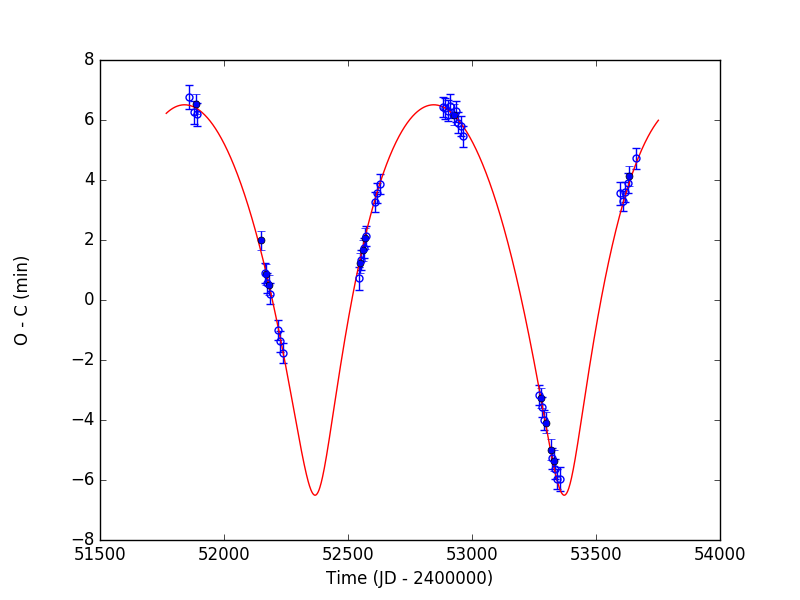
\includegraphics[width=\textwidth]{oc_1_5yrs.png}
        \caption{Star on equator.\\RA = 00:43:45.0838, DEC = +00:00:00}
    \end{subfigure}%
    \begin{subfigure}[t]{0.5\textwidth}
        \centering
        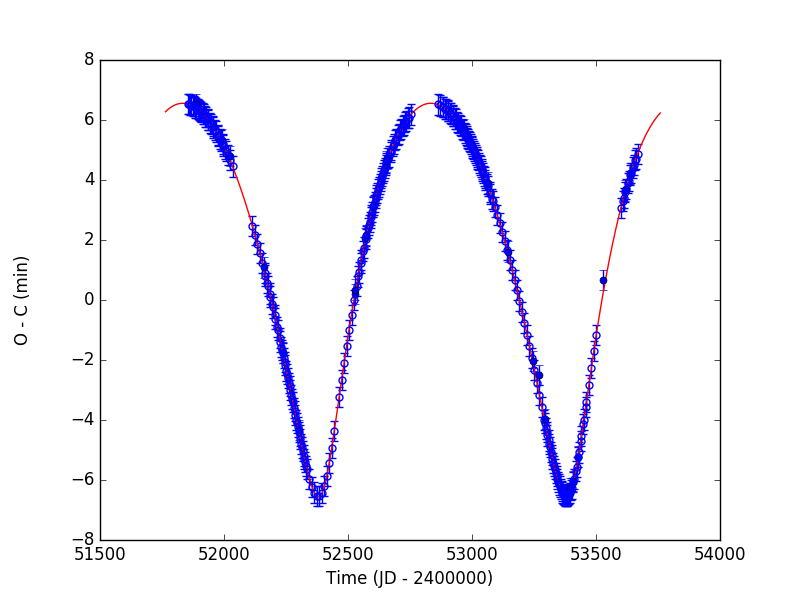
\includegraphics[width=\textwidth]{oc_2_5yrs.png}
        \caption{Star near north pole.\\RA = 00:43:45.0838, DEC = +89:30:00}
    \end{subfigure}
    \caption{O-C diagram for ideal conditions. Red line - fit with MCMC method, correspond to values in table \ref{tab:3rd_body_par}. Filled circles are primary minima, not filled circles - secondary minima. 
    Observatory is Kolonica AO \\(Lat = +48.934917, Lon = 22.2738)}
\label{fig:oc_1}
\end{figure}

\begin{table}[!h]
 \caption{Original parameters of the 3$^{rd}$ body orbit and parameters obtained by fitting $O-C$ diagram simulated in ideal condition on equator and near pole. $P$ -- orbital period of eclipsing pair, $T_0$ -- initial minimum, $P_3$ - orbital period of the 3$^{rd}$ body, $t_{03}$ -- pericenter passage, $a\sin i_3$  -- projected semi-major axis of the orbit, $e_3$ -- eccentricity, $\omega_3$ -- the longitude of the periastron, $f(M_3)$ -- the mass function, $\chi^2$ -- sum of squares of the best fit, $\chi^2/n$ -- reduced sum of squares ($n$ -- number of data points), errors are given in parenthesis.}
 \vspace{-6mm}
 \begin{center}
  \begin{tabular}{lccc}
    \hline
	Solution			& Original		    		& Equator				&  near Pole	\\
  \hline\noalign{\smallskip} 
 $P$ [days]				& 1.42834       			& fixed					& fixed	\\ 
 $T_0$ [HJD]			& 2451852.3783  			& fixed  				& fixed	\\
   \hline\noalign{\smallskip} 
 $P_3$ [days]   		&   1000 	    			& 997(3)				& 999.90(92)\\
 $t_{03}$ [HJD]			& 2451400       			& 2451407(9) 			& 2451400(1)	\\
$a\sin i_3$ [AU]		&  0.797 	 				& 0.807(15)				& 0.8001(35)\\
 $e_3$     				&  0.54				    	& 0.55(1)		 		& 0.5449(45)\\
$\omega_3$ [\degree] 	&   288 					& 289(3)			 	& 288.16(76)\\
\hline\noalign{\smallskip}
$f(M_3)$  [M$_\odot$]	&  --	  					& 0.070(4)				& 0.06835(91)\\
\hline\noalign{\smallskip}
$\chi^2$ 				&  --						& 8.34		 			& 8.323\\
$\chi^2/n$				&  --						& 0.19					& 0.026\\
\hline\noalign{\smallskip}
\end{tabular}
\end{center}
\label{tab:3rd_body_par}
\vspace{-6mm}
\end{table}

\subsection{Weather and Photometry Precision}
If we will take into account other factors, like weather and precision of photometry, we will get less fit accuracy. 
On the Fig.\ref{fig:oc_weather} (a, b) are presented O-C diagrams with same EB system as in previous case but now we take into account only 45\% of good weather, and photometry precision 0.0001. Such weather condition are rather good for our latitudes, photometry precision 0.0001 can be achieved on 400-600 mm telescopes with modern CCD cameras. Obtained parameters of $3^{rd}$ body orbit are presented in table \ref{tab:3rd_body_w}.

As we can se in table \ref{tab:3rd_body_w}, for a case when star is on equator difference with ideal condition is not so big on $\chi^2/n$ but accuracy of individual parameters is worse. It is because there is not much data point at all for this case.
On the other hand situation for a case when star is near the pole, in comparison with ideal conditions, is getting much worse. 

If we do a simulation of O-C diagrams with more appropriate for our latitudes 30 \% probability of clear sky, values are getting worse. This results are presented on Fig. \ref{fig:oc_weather} (c,d) and in table \ref{tab:3rd_body_w}.

In real life for research of some EB system light curves from many different observatories are used. If this observatories are situated on different latitudes then we will not have such big gaps in our data as can be seen for a case of star on equator. The more observatories contribute to research the less important is influence of weather conditions and object location.
% Weather and photom precision-----------------------------------------
\begin{figure}[!h]
    \centering
    \begin{subfigure}[t]{0.5\textwidth}
        \centering
        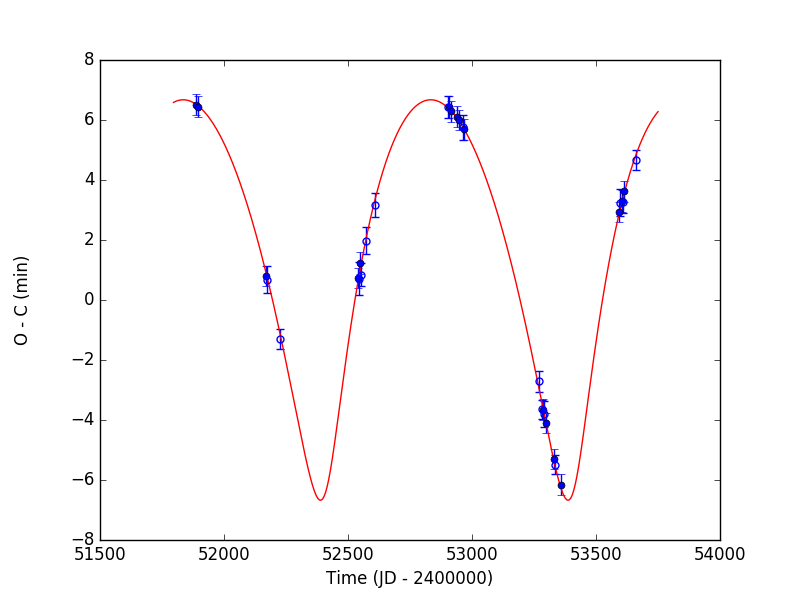
\includegraphics[width=\textwidth]{oc_w.png}
        \caption{Star on equator. 45\% of clear nights.\\RA = 00:43:45.0838, DEC = +00:00:00}
    \end{subfigure}%
    \begin{subfigure}[t]{0.5\textwidth}
        \centering
        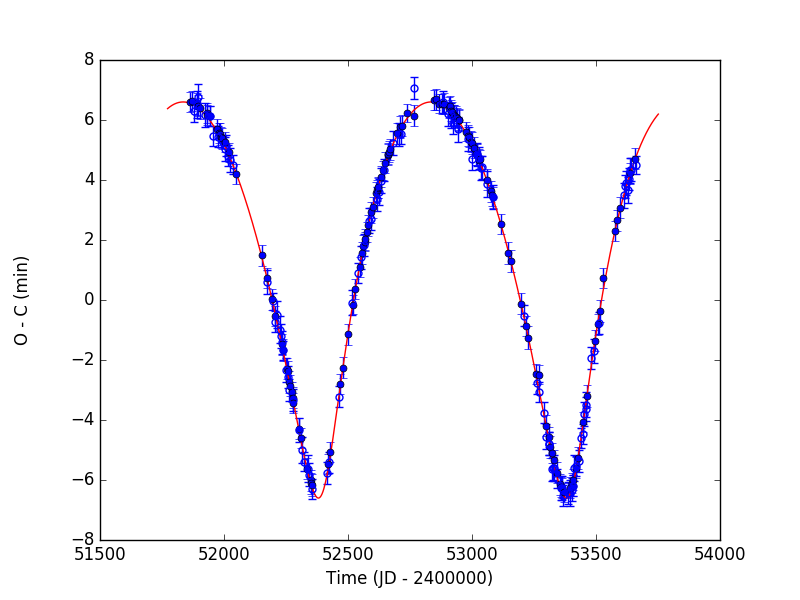
\includegraphics[width=\textwidth]{oc_eq_w2.png}
        \caption{Star near north pole. 45\% of clear nights\\RA = 00:43:45.0838, DEC = +89:30:00}
    \end{subfigure}
    
    \begin{subfigure}[t]{0.5\textwidth}
        \centering
        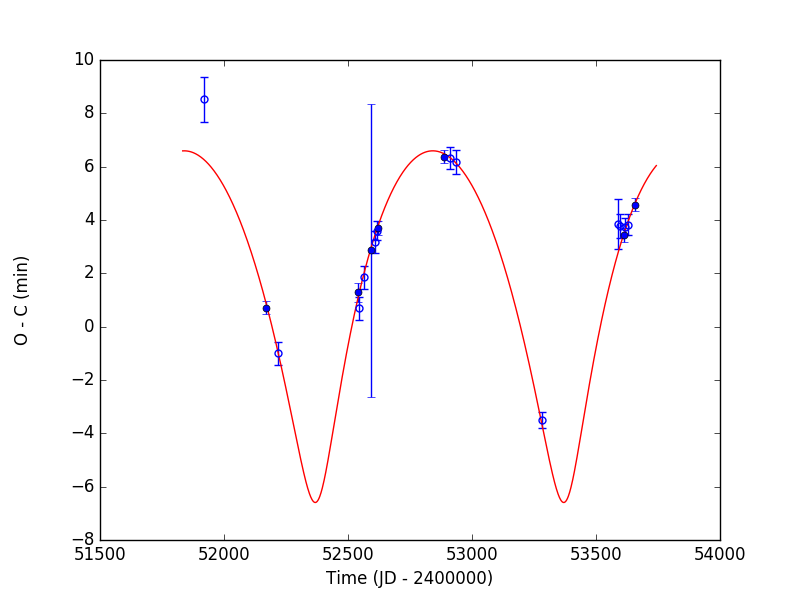
\includegraphics[width=\textwidth]{oc_w30_e.png}
        \caption{Star on equator. 30\% of clear nights\\RA = 00:43:45.0838, DEC = +00:00:00}
    \end{subfigure}%
    \begin{subfigure}[t]{0.5\textwidth}
        \centering
        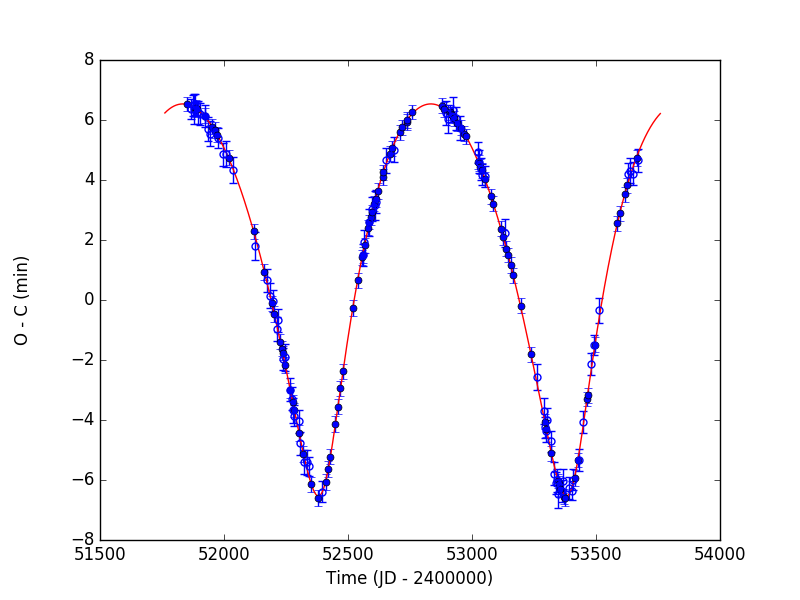
\includegraphics[width=\textwidth]{oc_w30_p.png}
        \caption{Star near north pole. 30\% of clear nights\\RA = 00:43:45.0838, DEC = +89:30:00}
    \end{subfigure}
    \caption{O-C diagram for 45\% (a,b) and 30\% (c,d) of good weather and photometry accuracy 0.0001.
    Red line - fit with MCMC method, correspond to values in table \ref{tab:3rd_body_w}. Filled circles are primary minima, not filled circles - secondary minima. Observatory is Kolonica AO \\(Lat = +48.934917, Lon = 22.2738)}
\label{fig:oc_weather}
\end{figure}


\begin{table}[!h]
 \caption{Original parameters of the 3$^{rd}$ body orbit and parameters obtained by fitting $O-C$ diagram simulated with influence of weather (45\% and 30\% of clear nights) and photometry precision 0.0001. For description of parameters see Table \ref{tab:3rd_body_par}}
 \vspace{-6mm}
 \begin{center}
  \begin{tabular}{lccccc}
    \hline
    Solution            & Original                  & Equator 45 \%         &  Pole 45\%          & Equator 30\%  &  Pole 30\%        \\
  \hline\noalign{\smallskip}                                                                                                                 
 $P$ [days]             & 1.42834                   & fixed                 & fixed               & fixed        & fixed             \\ 
 $T_0$ [HJD]            & 2451852.3783              & fixed                 & fixed               & fixed        & fixed             \\
   \hline\noalign{\smallskip}                                                                                                         
 $P_3$ [days]           &   1000                    & 998(4)                & 1000(1)             & 1002(5)      & 999(1)            \\
 $t_{03}$ [HJD]         & 2451400                   & 2451413(11)           & 2451398(3)          & 2451376(16)  & 2451399(3)       \\
$a\sin i_3$ [AU]        &  0.797                    & 0.819(22)             & 0.805(4)            & 0.797(22)    & 0.801(5)          \\
 $e_3$                  &  0.54                     & 0.553(14)             & 0.5588(57)          & 0.569(23)    & 0.558(6)        \\
$\omega_3$ [\degree]    &   288                     & 291(5)                & 287.6(9)            & 280(5)       & 289(1)          \\
\hline\noalign{\smallskip}                                                                                                                   
$f(M_3)$  [M$_\odot$]   &  --                       & 0.074(6)              & 0.069(1)            & 0.067(6)     & 0.069(1)          \\
\hline\noalign{\smallskip}                                                                                                               
$\chi^2$                &  --                       & 4.82                  & 36.46               & 15.00        & 31.29              \\
$\chi^2/n$              &  --                       & 0.18                  & 0.16                & 1.00         & 0.18              \\
\hline\noalign{\smallskip}

\end{tabular}
\end{center}
\label{tab:3rd_body_w}
\vspace{-6mm}
\end{table}

\subsection{Spots in EB Systems}
In previous chapters we was dealing with terrestrial factors that cause inaccuracy in O-C diagrams. 
Now we will try to simulate O-C diagrams in ideal terrestrial conditions but under influence of other non-terrestrial factor like star spots.

As we know formation of star spots depends on a age of a host star, that's why we should separate our simulation on detached and over-contact EB systems.  
But before we start to simulate we need to know some general spot parameters for this EB systems. Its a radius of star spot, its temperature, and life cycle. Do the spot disappear after some short time or can be present on a host star for a relative long time like 5-10 years? The spots migrate or not?   

In \cite{Watson2004} authors said that depressed star-spots also cause a jitter in the residuals of O-C
diagrams, which can also result in the false detection of spurious orbital period changes. Such changes resulting from star-spots
would be distinguishable from other mechanisms that cause period
changes and it should still be possible to determine the orbital period accurately.

In previous work \cite{Kalimeris2002} authors have
shown that intensity variations resulting from star-spots (not taking into account Wilson depressions) can introduce disturbances of
up to $\sim 0.01~day$ in the O-C residuals of contact binaries. Given the
rapid evolutionary time-scales of spots (of the order of days) seen in
recent Doppler images of the contact binary AE Phe \citep{Barnes2004} 
this may lead to explaining some of the observed jitter in the
O-C curves of these objects. But in work \cite{Watson2004}, the effects of a
Wilson depression seem to result in a scatter of only a few seconds
in the O-C residuals, it seems unlikely that the Wilson depression
will be a significant source of jitter for contact binaries \citep{Watson2004}.

Several studies have indicated that spot  on close binaries can have angular diameters from $10\degree$ to $40\degree$ which means that they
will cover from 5 to 25\% of the whole photosphere of the active components (e.g. \cite{Hall1990, Guinan1993}).
In most cases, active component can have one or two giant spots. It is also argued that such spots can remain on a surface from few years to even ten years \citep{Kalimeris2002}. 

For a estimation of maximum effect caused by the star spot, it is assumed that in our simulations spots are located on equator of each component.
According to \cite{Kalimeris2002} spots with angular diameter less then $10\degree$ cause negligible shifts of the light minimum of the primary eclipse. Therefore we will not consider with spots smaller then $10\degree$ (see fig. \ref{fig:spot_diam}).

Furthermore, the spots on secondary component always remain visible during the primary eclipse,
while the spots on primary do not. As a result, the spots on primary cause a
significantly greater photometric perturbation to the light curve than the spots on secondary component.

\citeauthor{Kalimeris2002} also showed that unlike real orbital period changes, non-migrating star spots cannot
cause permanent slopes in the O-C diagrams. 
But the O-C differences caused by long-lived migrating spots can be expected to be periodic.

\begin{figure}[!h]
\vspace{0cm}
\centerline{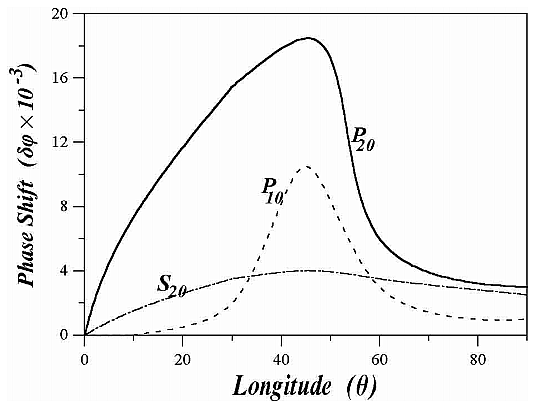
\includegraphics[width=0.60\textwidth]{spot_diam_2.png}}
\caption{Phase shift $\delta\varphi(\theta)$ of the primary eclipse of a contact
binary similar to AB And. Curves labelled by "P" correspond
to a spot on the primary, while "S" refers to a spot on the
secondary component \cite{Kalimeris2002}.}
\label{fig:spot_diam}
\end{figure}   
 

\subsubsection{Detached EB Systems}
% Pro single stars
%Younger stars rotate faster than older stars and
%have higher activity levels and greater spot coverage (????). As a result, there is an overall trend of the
%degree of photometric variability with age. % \cite article "The Ages of Stars".

Tidal interactions force most of these stars to rotate synchronously with their orbital motions. 
The rapid rotation combined with deep convection envelopes produces a variety of magnetic activity phenomena including starspots in
these stars.

Brightness variations due to starspots can be observed in detached EB only during primary total
eclipses, when the luminous hot components are hidden. Therefore, because of synchronised rotation, 
only one hemisphere of the cool stars can be observed and the photometric data
collected are less detailed than for other spotted binaries \citep{Berdyugina2005}.
 
For detached eclipsing binary systems spots with radius from 5\degree~to~25\degree are usually typical, we can find such systems in a many publications like e.g. \cite{Liakos2011} or in publications about spot for RSCVn binaries systems (e.g. \cite{Roettenbacher2011, Kovari2012, Kozhevnikova2015}). Objects with spots migrations are very rarely observed, so we will not consider such case.
Model of detached EB system is presented on figure \ref{fig:eb_det_model}, main parameters of this system is listed in table \ref{tab:detached_params}.

As we mentioned above, spots with radius less then 10\degree~ do not have big influence on O-C diagram. So, we will consider how star spot located on stars equator (colat=90\degree, lon=0\degree) with radius $r_{spot}=15\degree$ and $r_{spot}=25\degree$~ affect the O-C diagram. 
There is also a difference in hot and cold spot. Hot spot will have $T_{spot}=1.2$, where $T_{spot}$ is the ratio between the temperature of the
spot and the local temperature of the underlying photosphere, cold spot will be defined as $T_{spot}=0.8$. On figure \ref{fig:detached_spots} we can see how hot and cold spots affect the shape of the minima. Mainly primary minima is changing its shape under the influence of spots.

\begin{figure}[!h]
\vspace{0cm}
\centerline{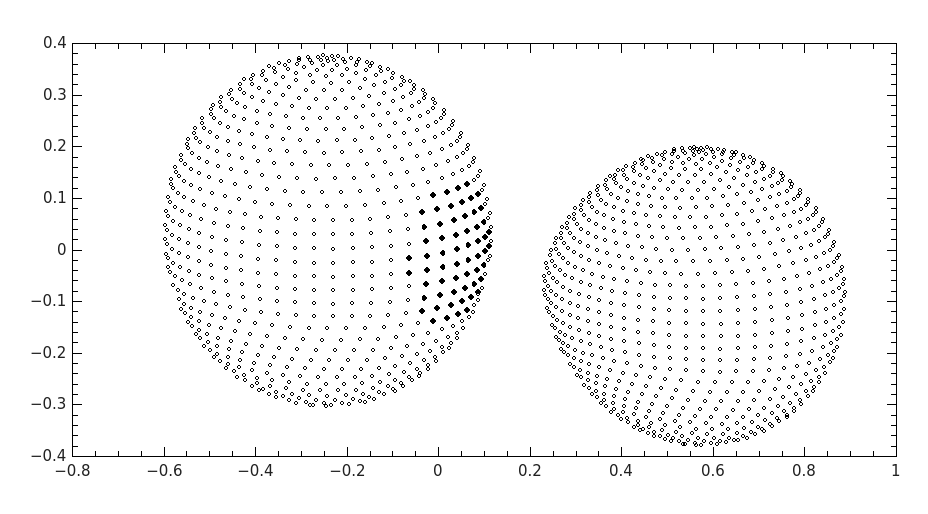
\includegraphics[width=0.80\textwidth]{detached_pspot_08-25_view.png}}
\caption{Model of detached EB system with spot (colat=90\degree, colon=0\degree) in plane of sky view at phase 0.15.}
\label{fig:eb_det_model}
\end{figure}

\begin{table}[!h]
 \caption{Basic parameters of detached binary system presented on figure~ \ref{fig:eb_det_model}. HJD0 is a origin of the
 ephemeris; P - orbital period of EB system; SMA - semi-major axis; RM - mass ratio; VGA - centre of mass velocity, \\INCL - inclination}
 \begin{center}
 \vspace{-6mm}
  \begin{tabular}{c|c}
    \hline 
HJD0(day) & 2451852.3783\\
P(day)    & 1.42834\\
\hline
SMA ($R_\odot$) &  1.000\\
RM              &  0.432\\
VGA (km/s)      &  0\\
INCL (\degree)  & 77.690\\
\hline
\end{tabular}
\end{center}
\label{tab:detached_params}
\vspace{-6mm}
\end{table}

\begin{figure}[!h]
    \centering
    \begin{subfigure}[t]{0.5\textwidth}
        \centering
        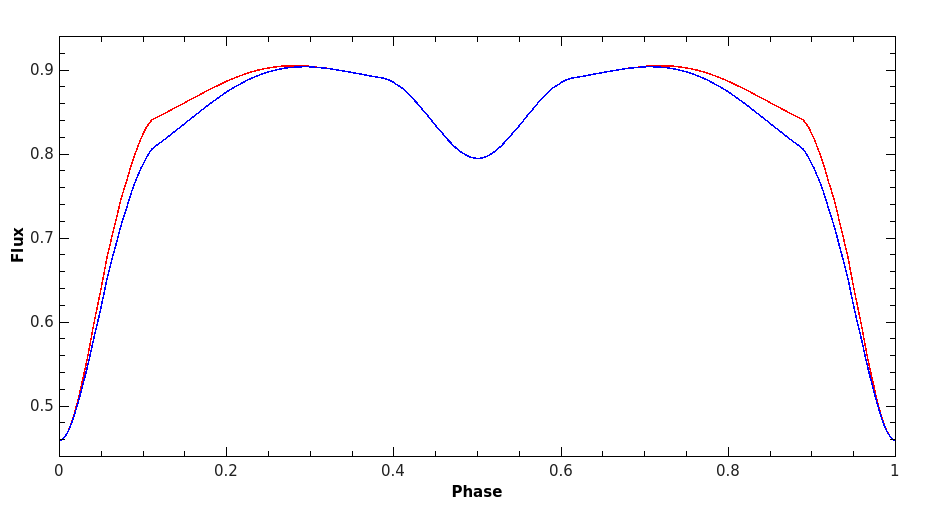
\includegraphics[width=\textwidth]{detached_pspot_08.png}
        \caption{Spot with $T_{spot}=0.8$}
    \end{subfigure}%
    \begin{subfigure}[t]{0.5\textwidth}
        \centering
        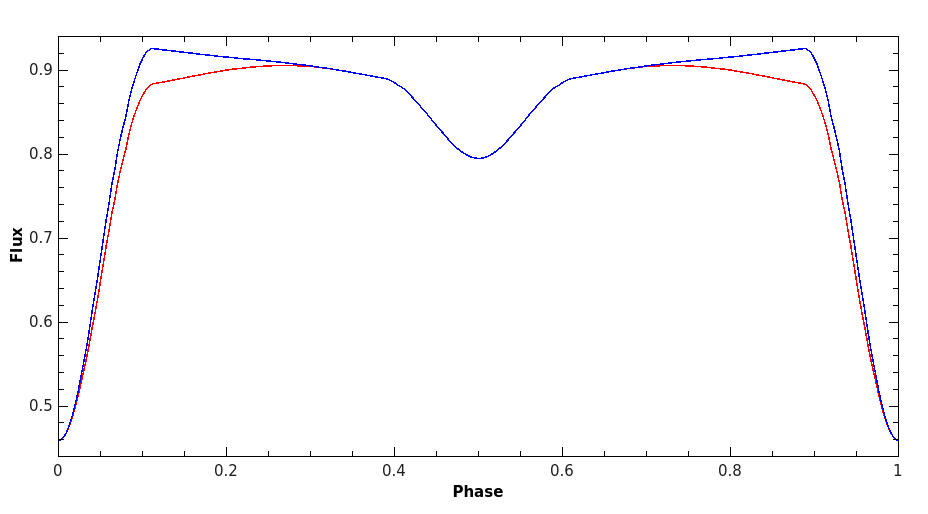
\includegraphics[width=\textwidth]{detached_pspot_12.png}
        \caption{Spot with $T_{spot}=1.2$}
    \end{subfigure}
    \caption{Spot on primary component with different temperature and radius. 
    Blue line - spot radius 25\degree, red line - spot radius 15\degree}
\label{fig:detached_spots}
\end{figure}

The final O-C diagrams for all four cases are presented on figure \ref{fig:oc_detached_spot}. Looking only on O-C diagram we can't clearly see the difference. Only when we fit this O-C diagrams by MCMC method results are getting clearer. 
Final results of fitting are presented in table \ref{tab:3rd_body_detached_spot}. The $\chi^2$ value of 4 cases are almost the same, except case of spot with $T_{spot}=1.2$ and $R_{spot}=25\degree$, in this case $\chi^2$ is the best. 
%But if we take into account Bayesian information criterion (BIC) and Akaike information criterion (AIC), where bigger value corresponds to better fit, the situation changes to the opposite. 
Best fit is case with small cold spot, and worst fit is case with hot and big spot.\\
(RECALCULATE!!!!!) 

\begin{figure}[!h]
    \centering
    \begin{subfigure}[t]{0.5\textwidth}
        \centering
        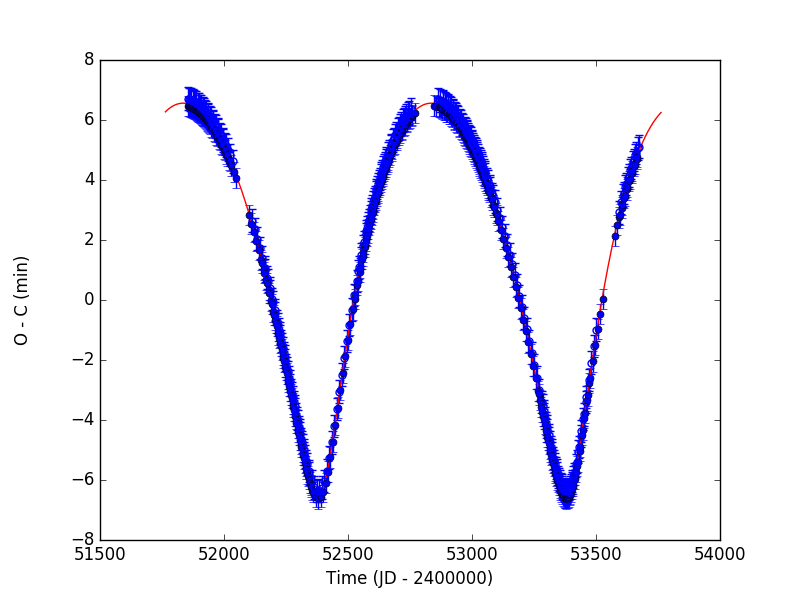
\includegraphics[width=\textwidth]{oc_detached_pspot_R15_T12.png}
        \caption{O-C diagram with $R_{spot}=15, T_{spot}=1.2$}
    \end{subfigure}%
    \begin{subfigure}[t]{0.5\textwidth}
        \centering
        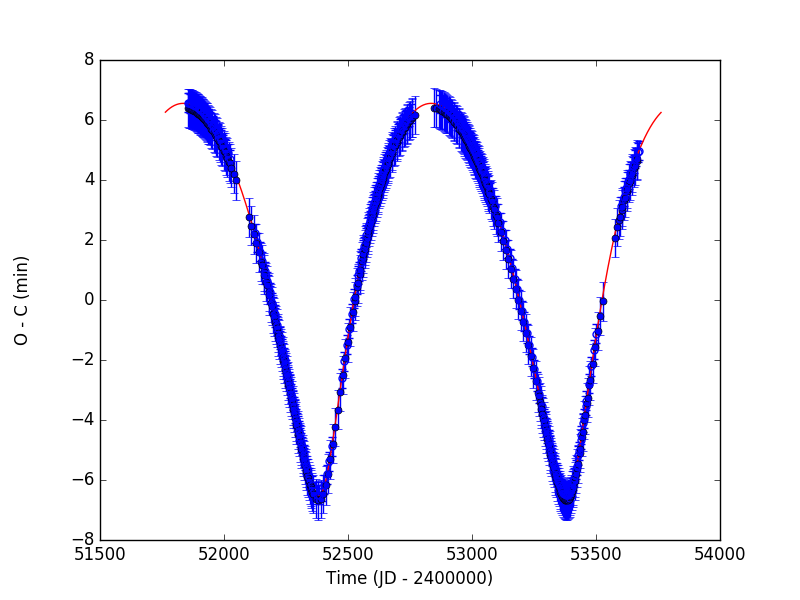
\includegraphics[width=\textwidth]{oc_detached_pspot_R25_T12.png}
        \caption{O-C diagram with $R_{spot}=25, T_{spot}=1.2$}
    \end{subfigure}
    
    \begin{subfigure}[t]{0.5\textwidth}
        \centering
        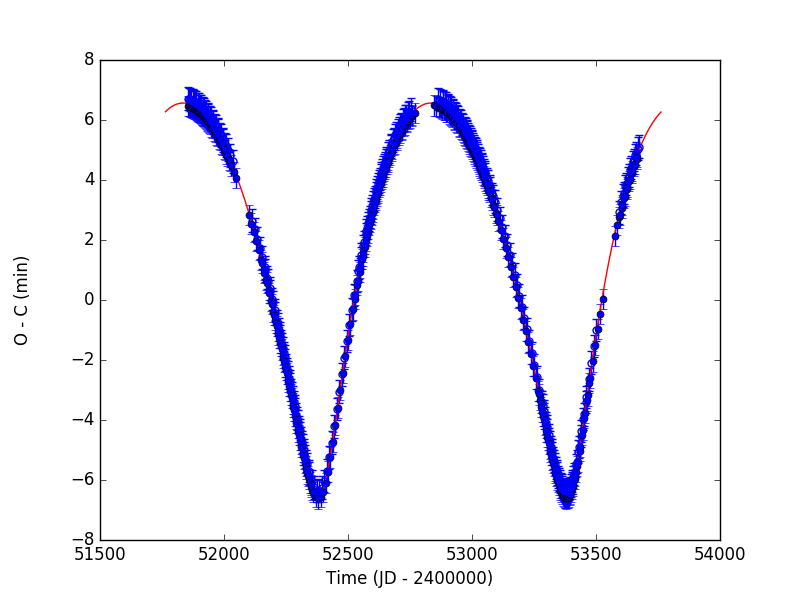
\includegraphics[width=\textwidth]{oc_detached_pspot_R15_T08.png}
        \caption{O-C diagram with $R_{spot}=15, T_{spot}=0.8$}
    \end{subfigure}%
    \begin{subfigure}[t]{0.5\textwidth}
        \centering
        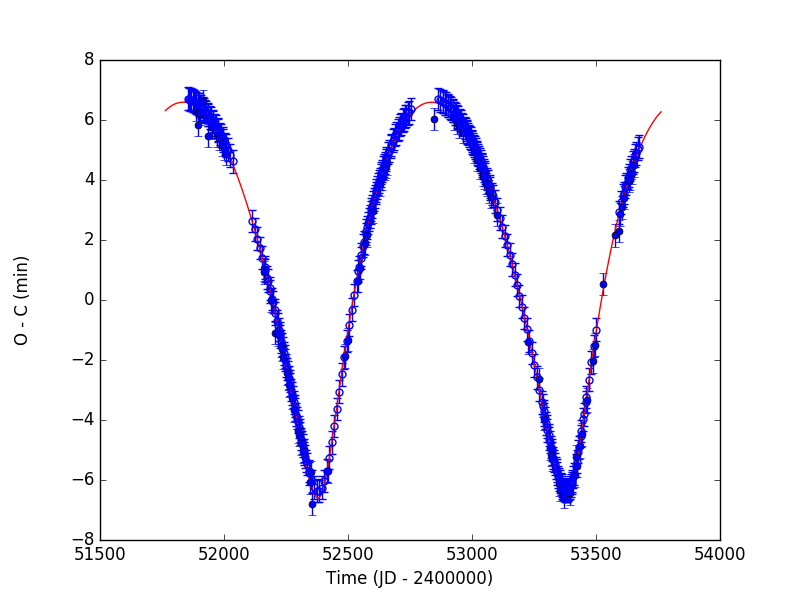
\includegraphics[width=\textwidth]{oc_detached_pspot_R25_T08.png}
        \caption{O-C diagram with $R_{spot}=25, T_{spot}=0.8$}
    \end{subfigure}
    \caption{O-C diagram for EB system with different $R_{spot}$ and $T_{spot}$\\
    Red line - fit with MCMC method, correspond to values in table \ref{tab:3rd_body_detached_spot}. 
    Filled circles are primary minima, not filled circles - secondary minima.}
\label{fig:oc_detached_spot}
\end{figure}


\begin{table}[!h]
 \caption{Orbital parameters of $3^{rd}$ body for detached EB system with different spot parameters $R_{spot}$ and $T_{spot}$. 
 For description of parameters see Table~\ref{tab:3rd_body_par}}
  \vspace{-6mm}
 \begin{center}
  \begin{tabular}{lccccc}
    \hline
    Solution            & Original       & $R_{spot}$=25\degree&$R_{spot}$=25\degree  &$R_{spot}$=15\degree &$R_{spot}$=15\degree \\
                        &                &    $T_{spot}$=1.2    &  $T_{spot}$=0.8 &  $T_{spot}$=1.2  &  $T_{spot}$=0.8 \\
  \hline\noalign{\smallskip}                                                                                                                 
 $P$ [days]             & 1.42834        &           fixed     & fixed       & fixed        & fixed       \\ 
 $T_0$ [HJD]            & 2451852.3783   &           fixed     & fixed       & fixed        & fixed       \\
   \hline\noalign{\smallskip}                                                                                                         
 $P_3$ [days]           &   1000         &          999.9(9)   & 1001(1)     &   1000.7(9)  &  999.8(7)   \\       
 $t_{03}$ [HJD]         & 2451400        &          2451400(2) & 2451394(2)  &   2451397(2) &  2451400(1) \\
$a\sin i_3$ [AU]        &  0.797         &          0.799(3)   & 0.803(3)    &   0.799(3)   &  0.801(2)   \\     
 $e_3$                  &  0.54          &          0.541(4)   & 0.566(5)    &   0.548(3)   &  0.547(3)   \\            
$\omega_3$ [\degree]    &   288          &          287.8(7)   & 286.6(8)    &   287.4(8)   &  288.0(5)   \\     
\hline\noalign{\smallskip}                                                                                                 
$f(M_3)$  [M$_\odot$]   &  --            &          0.0681(8)  & 0.0689(9)   &   0.0681(7)   &  0.0686(7)  \\       
\hline\noalign{\smallskip}                                                                                             
$\chi^2$                &  --            &          21.714     & 54.867      &  74.652      &  74.168     \\        
$\chi^2/n$              &  --            &           0.0347    & 0.1432      &   0.1161     &   0.1153    \\       
% AIC                    &  --            &          31.714     & 64.867      &  84.652      &  84.168     \\
% BIC                    &  --            &          53.942     & 84.672      & 107.022      & 106.538     \\
\hline\noalign{\smallskip}  

\end{tabular}
\end{center}
\label{tab:3rd_body_detached_spot}
\vspace{-6mm}
\end{table}

It was mentioned above that spot on secondary component do not have a big influence on minima shape, so we will not consider here this option.

As conclusion we can say that detached EB systems with spot are not sophisticated objects for $3^{rd}$ body detection. In case of bigger then 25\degree ~spots on surface it is advisable to cut off from the top the height of primary (or secondary) minima to get better fit and to determine time of minima more precisely.
 
\subsubsection{Contact EB Systems}
Contact binary stars occur relatively often among binaries (95\% of eclipsing binary
variables in the solar neighbourhood) \cite{Rucinski98}. 
A contact binary system consists of two dwarf stars, most often from the F, G, and K
spectral classes, that are surrounded by a common convective envelope. 
The orbital period distribution peaks in the 8 to 12 hour range. Most systems, though not all,
have orbital periods between 0.2 and 1.0 days \citep{Maceroni96, Paczynski2006}. 
While the masses of the two component stars of a contact binary
are typically unequal, the two stars usually have approximately equal surface temperatures due to the effects of
mass and energy transfer between the components via a common convective envelope \citep{Lucy68}. 
Eclipsing contact binaries are often referred to as W UMa systems in honor of the prototype \citep{Tran2013}.

The components of such a contact binary rotate very rapidly in spite of their old ages
($v~sin~i \sim 100 - 200~ km~s^{-1}$ ) as a result of spin-orbit synchronisation due to strong tidal interactions between the stars. 

%Observations reveal that there are two subclasses of W UMa stars: A-type and W-type systems.
%The former have longer periods, are hotter, have larger total mass, and a smaller mass-ratio and
%are in better contact.
Many contact binaries show signs of stellar activity, presumably because the component stars are rapid
rotators with deep convective zones. 
A study of the contact binaries with Doppler imaging
technique reveals that both components can be covered by cool starspots, with
a tendency for the primary to be more active than the secondary \citep{Maceroni94, Hendry2000, Barnes2004}.

This makes contact binaries excellent laboratories in
which to investigate the temporal variations and evolution of stellar spots, in part because the timescales of
the variations are shorter than in other types of binary and single stars. 
However, the shortest among these timescales can be problematic to study using groundbased observatories because they are comparable to the
length of an Earth night.

\begin{figure}[!h]
\vspace{0cm}
\centerline{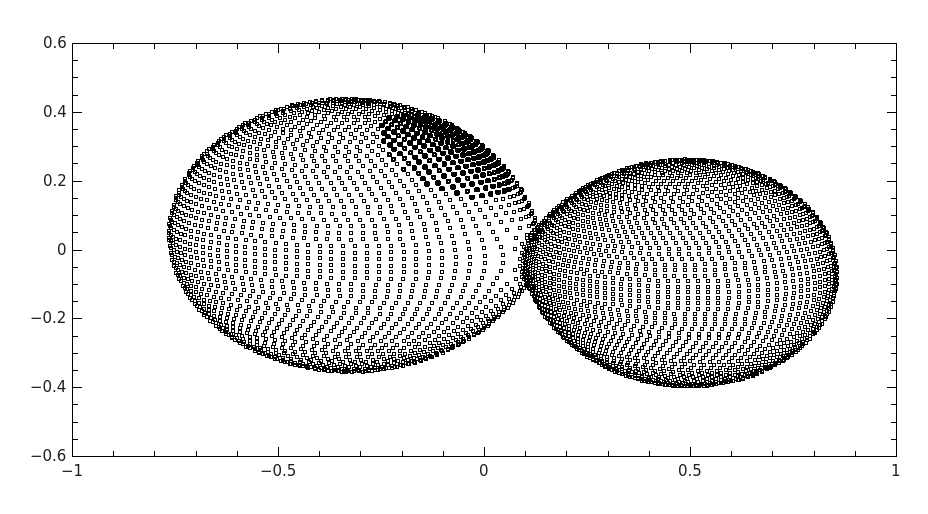
\includegraphics[width=0.8\textwidth]{Overcontact_mesh.png}}
\caption{Model of overcontact EB system with spot (colat=45\degree, colon=0\degree) in plane of sky view at phase 0.15.}
\label{fig:eb_overcont_model}
\end{figure}


\begin{table}[!h]
 \caption{Baisic parameters of overcontact binary system presented on figure~ \ref{fig:eb_overcont_model}. HJD0 is a origin of the
 ephemeris; P - orbital period of EB system; SMA - semi-major axis; RM - mass ratio; VGA - centre of mass velocity, \\INCL - inclination}
 \begin{center}
 \vspace{-6mm}
  \begin{tabular}{c|c}
    \hline 
HJD0(day) & 2451852.3783\\
P(day)    & 1.42834\\
\hline
SMA ($R_\odot$) &  1.76\\
RM              &  0.67\\
VGA (km/s)      &  4.70\\
INCL (\degree)  & 79.50\\
\hline
\end{tabular}
\end{center}
\label{tab:overcontact_params}
\vspace{-6mm}
\end{table}

\cite{Kalimeris2002} noted that the migration of
starspots on the surface(s) of the constituent stars in
short-period binaries, especially contact binaries, could
affect measurements of eclipse times and thereby mimic
changes in the orbital period. \cite{Kalimeris2002} also
showed that the perturbations to the O-C diagrams would generally have amplitudes smaller than $\sim 0.01$ days, and could appear to
be quasiperiodic on timescales of a few hundred days or so if the spot migration is related to differential rotation
of the host star \citep{Tran2013}.

Model of overcontact EB system with spot is presented on figure \ref{fig:eb_overcont_model}, orbital parameters can be found in table \ref{tab:overcontact_params}. 

\begin{figure}[!h]
    \centering
    \begin{subfigure}[t]{0.5\textwidth}
        \centering
        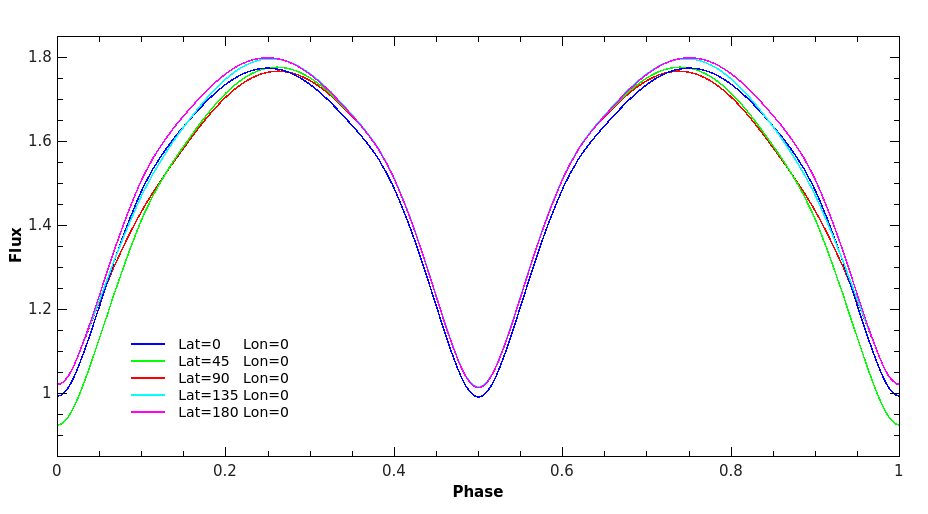
\includegraphics[width=\textwidth]{Overc_spot_pos_lat.png}
        \caption{LC with spot on different colatitude and \\longitude = 0\degree}
    \end{subfigure}%
    \begin{subfigure}[t]{0.5\textwidth}
        \centering
        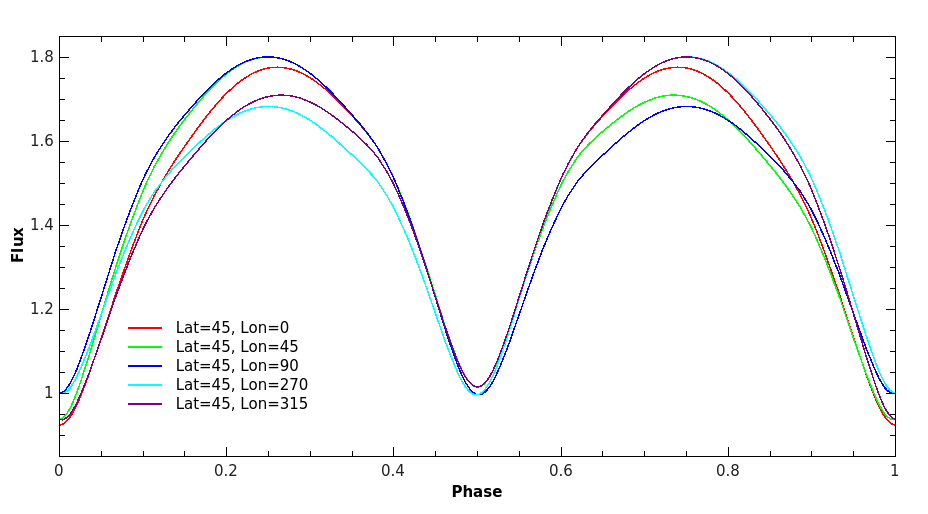
\includegraphics[width=\textwidth]{Overc_spot_pos_lon.png}
        \caption{LC with spot on different longitude and \\colatitude = 45\degree}
    \end{subfigure}
    \caption{LC of overcontact binary system with "cold" spot ($T_{spot}=0.8~T_{surf}$) on primary component at different positions}
\label{fig:overcontact_spot_pos}
\end{figure}

Light curve from such EB system will undergo changes depending on the position of the spot, such changes are partially presented on figure \ref{fig:overcontact_spot_pos}, \ref{fig:overcontact_spotT12_pos}. Analyzing these data we can conclude that the most noticeable changes in LC are caused by changes of position in longitude of a starspot on primary component of contact binary EB system.
If we change spot position only in colatitude and leave longitude = 0\degree, we will observe only variation of primary minima shape and depth. On the other hand if we make colatitude constant (colatitude = 45\degree~ on figures \ref{fig:overcontact_spot_pos}, \ref{fig:overcontact_spotT12_pos}) and change longitude of spot then in addition to the primary minimum part of the LC between two minima will vary too. As it can be expected "hot" spot has a greater contribution to changes in LC than "cold" spot (see fig \ref{fig:overcontact_spot_pos}b vs \ref{fig:overcontact_spotT12_pos}b). 

\begin{figure}[!h]
    \centering
    \begin{subfigure}[t]{0.5\textwidth}
        \centering
        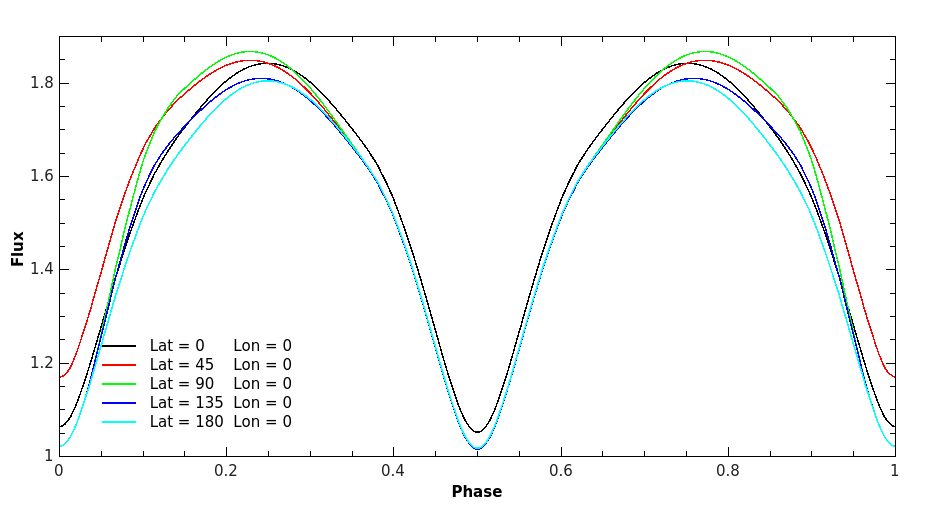
\includegraphics[width=\textwidth]{overc_spotT12_pos_lat.png}
        \caption{LC with spot on different colatitude and \\longitude = 0\degree}
    \end{subfigure}%
    \begin{subfigure}[t]{0.5\textwidth}
        \centering
        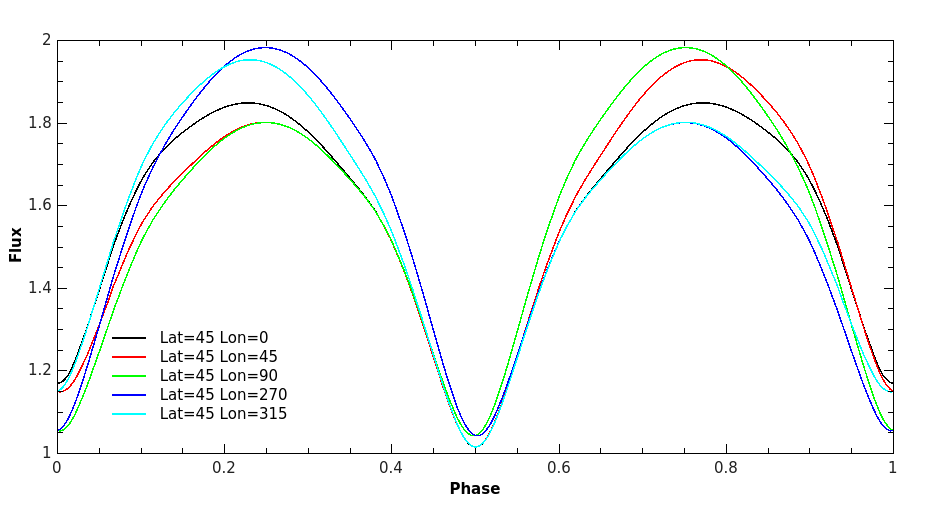
\includegraphics[width=\textwidth]{overc_spotT12_pos_lon.png}
        \caption{LC with spot on different longitude and \\colatitude = 45\degree}
    \end{subfigure}
    \caption{LC of overcontact binary system with "hot" spot ($T_{spot}=1.2~T_{surf}$) on primary component at different positions}
\label{fig:overcontact_spotT12_pos}
\end{figure}

From previous results with detached EB system we already know that bigger and hotter spot adds more uncertainty to definition of orbital elements $3^{rd}$ body available in EB system. We can expect same results with contact EB systems. So let us define a influence of spot migration and presence of spot on secondary EB component. This two aspects can be often found in contact and overcontact systems.
  
According to \cite{Kalimeris2002} rotation period of starspot differs from $P_{eq}$ by:
\begin{equation}
\Delta P = P_\lambda-P_{eq},  % = \frac{P_{eq} \cdot k \cdot \sin^2\lambda}{1-k \cdot \sin^2 \lambda}
\end{equation} 
where $P_{eq}$ is the equatorial period of rotation ($P_{eq}=P_0$), and $P_{\lambda}$ is a period of starspot rotation equal to:

\begin{equation}
P_\lambda = P_{eq} \cdot (1-k \cdot \sin^{2}\lambda)^{-1}, 
\label{eq:Pl}
\end{equation} 

in equation \ref{eq:Pl} $k$ is a coefficient of differential rotation. For close binaries observation have indicated a range between 
$k\approx 6 \times10^{-4}$ and 0.18 with mean value $\bar{k}=3 \times10^{-2}$ \citep{Hall1990}. At the end of each orbital cycle, a starspot will shift  in longitude by: 
\begin{equation}
\delta \theta = 2\pi \frac{\Delta P}{P}
\end{equation}

If we calculate this value for our EB system with period $P=1.42834$ which has spot on latitude $\lambda=45\degree$ and mean value of $k$ we will get $\delta \theta = 5.4798\degree$ or $\delta \theta \sim 5.5\degree$. So spot with such parameters will do a full revolution in $\sim 65.5$ cycles or in our case this is equal to 93.5 days. To simplify the process of simulation we take an integer number of $\delta \theta = 6\degree$ in such case the spot will do a full revolution in 60 cycles or in 85.7 days. 

Large spots causing prominent light curve minima apparently can survive for many years, despite differential rotation, and form centres
of activity, or active longitudes \citep{Berdyugina2005}. Polar spots are found to have lifetimes of over a decade \citep{Hussain2002}.
Our simulation of $3^{rd}$ body is made on 5 years time interval so lets define that our spot lifetime is also 5 years.

Last question that we need to know is a radius of a spot. Lets consider a case with a spot radius $35\degree$ because a bigger spots are more typical for this type of EB systems. 

 
\begin{figure}[!h]
    \centering
    \begin{subfigure}[t]{0.5\textwidth}
        \centering
        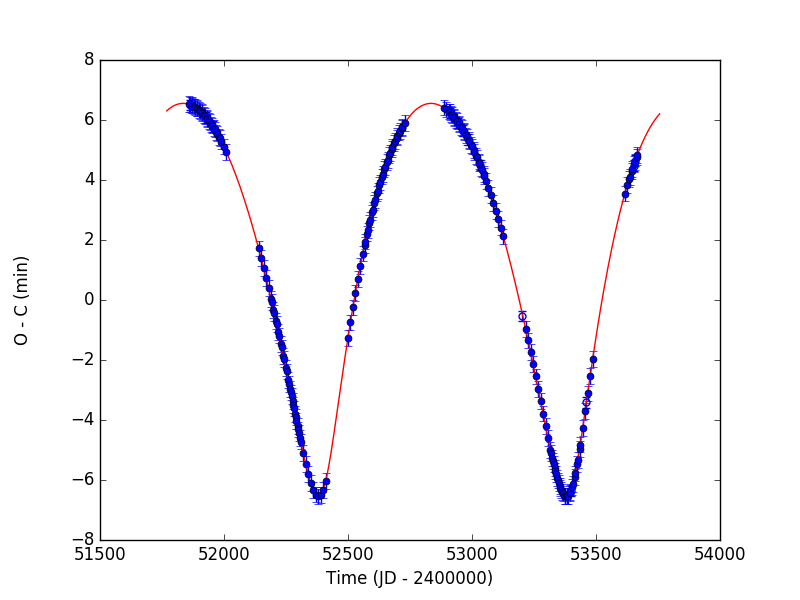
\includegraphics[width=\textwidth]{overc_ideal.png}
        \caption{o-c ideal}
    \end{subfigure}%
    \begin{subfigure}[t]{0.5\textwidth}
        \centering
        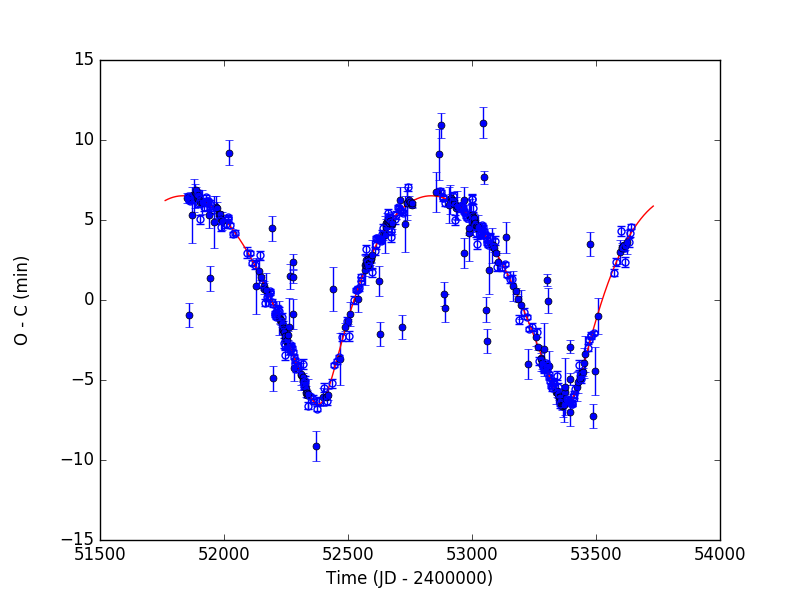
\includegraphics[width=\textwidth]{overc_spot_migr2.png}
        \caption{o-c with spot}
    \end{subfigure}
    \caption{O-C}
\label{fig:overcontact_spot_oc}
\end{figure}

From figure \ref{fig:overcontact_spot_oc} we can clearly see how migrated spot reduce precisions of minima exact time detection and in some cases we even got point that do not fit in our O-C diagram. This means that these point are faults. Migrated spots are the most difficult cases for precise definition time of minima, make O-C diagram and define orbital parameters of $3^{rd}$ body.
Fitted parameters of orbit and $\chi^2$ values of fit are presented in table \ref{tab:3rd_body_overc_spot}. 
  
\begin{table}[!h]
 \caption{Orbital parameters of $3^{rd}$ body for overcontact EB system with migrated spot. Spot parameters $R_{spot}=35\degree$, $T_{spot}=0.8~T_{surf}$. For description of parameters see Table~\ref{tab:3rd_body_par}}
  \vspace{-6mm}
 \begin{center}
  \begin{tabular}{lccc}
    \hline
    Solution            & Original       & no       & migrated   \\
                        &                & spot     & spot  \\
  \hline\noalign{\smallskip}                                                                                                                 
 $P$ [days]             & 1.42834        &           fixed     & fixed        \\ 
 $T_0$ [HJD]            & 2451852.3783   &           fixed     & fixed        \\
   \hline\noalign{\smallskip}                                                                             
 $P_3$ [days]           &   1000         &          999.7(8)   & 1000(1)      \\       
 $t_{03}$ [HJD]         & 2451400        &          2451400(2) & 2451398(4)   \\
$a\sin i_3$ [AU]        &  0.797         &          0.799(3)   & 0.764(3)     \\     
 $e_3$                  &  0.54          &          0.541(4)   & 0.541(2)     \\            
$\omega_3$ [\degree]    &   288          &          288.1(7)   & 287(1)     \\     
\hline\noalign{\smallskip}                                                                     
$f(M_3)$  [M$_\odot$]   &  --            &          0.0681(8)  & 0.0666(7)    \\       
\hline\noalign{\smallskip}                                                                 
$\chi^2$                &  --            &          0.614      & 2478.629      \\        
$\chi^2/n$              &  --            &          0.0283     & 6.1200       \\       
% AIC                    &  --            &          10.614     & 2488.629       \\
% BIC                    &  --            &          27.628     & 2508.709      \\
\hline\noalign{\smallskip}  

\end{tabular}
\end{center}
\label{tab:3rd_body_overc_spot}
\vspace{-6mm}
\end{table}

\subsection{Pulsations in EB Systems}
Pulsation in eclipsing binary systems can be observed in Algol-type binaries, the so-called oEA stars (oscillating EA stars).
The oEA stars are mass-accreting mainsequence A/F-type components in semidetached Algol-type eclipsing binary systems showing $\delta$~Sct - like pulsation \citep{Rodriguez2010}. The period of pulsation in such systems can vary from 20 to 300 minutes (see e.g \cite{Liakos2017}, \cite{Mkrtichian2007}). 

In work \cite{Liakos2017} relation for period of pulsation is given as:
\begin{equation}
P_{pul} = 0.031(4) + 0.009(1) P_{orb}. 
\end{equation} 

This relation is based on observation of $\delta$~Sct stars in all known close binaries systems (Detached, Semi-detached, unclassified). Coefficient of correlation for this relation is $r = 0.62$.

To determine how the pulsations affect the O-C diagram and $3^{rd}$ precision of orbital elements we will consider three cases of detached EB systems with different period of pulsations: 30, 150, 300 minutes.

To determine precise time of minima with pulsation presence it is very important have high rate of observation per some time interval.
Until now we use synthetic LC generated by PHOEBE with sample rate 300 point per period. This rate is not enough for pulsation study.
To determine what sample rate should we use lets see what results we will obtain in detached EB system with added pulsations with period $P_{pus}=30$ min and amplitude $A_{puls} = 0.02$.           
